\SourceLeaf{235}%
\Needspace{12\baselineskip}
\begin{center}[III.]\end{center}
\begin{center}\textsc{Cubirung der Tetraeder.}\end{center}
Im Tetraeder $1234$ sind die Seitenflächen $124$ gegen $134$ senkrecht. Der Inhalt $=\Delta$.
\begin{center}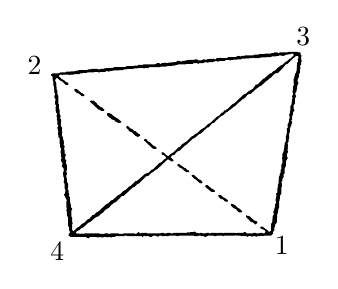
\begin{tikzpicture}[x=0.00720721cm,y=-0.00720721cm]
\fill[even odd rule] (508,63) -- (507,62) -- (504,62) -- (503,61) -- (486,61) -- (485,62) -- (471,62) -- (470,63) -- (468,63) -- (467,62) -- (462,62) -- (461,63) -- (457,63) -- (456,64) -- (445,64) -- (444,65) -- (435,65) -- (434,66) -- (426,66) -- (425,67) -- (410,67) -- (409,68) -- (404,68) -- (403,69) -- (397,68) -- (394,70) -- (381,70) -- (378,72) -- (368,72) -- (366,71) -- (365,72) -- (360,72) -- (358,74) -- (356,74) -- (355,73) -- (343,74) -- (342,75) -- (337,74) -- (333,76) -- (328,76) -- (325,74) -- (322,74) -- (321,75) -- (309,75) -- (308,76) -- (305,76) -- (304,77) -- (299,77) -- (298,78) -- (296,78) -- (295,77) -- (291,77) -- (288,79) -- (275,80) -- (274,81) -- (268,80) -- (267,81) -- (263,81) -- (262,82) -- (260,82) -- (259,81) -- (255,81) -- (251,83) -- (231,83) -- (230,84) -- (222,84) -- (221,85) -- (215,85) -- (214,86) -- (202,86) -- (198,88) -- (179,88) -- (178,89) -- (162,90) -- (161,91) -- (155,91) -- (154,92) -- (151,92) -- (150,91) -- (139,91) -- (138,92) -- (133,92) -- (132,93) -- (117,93) -- (116,94) -- (113,94) -- (112,95) -- (95,96) -- (94,97) -- (85,97) -- (81,99) -- (71,99) -- (70,100) -- (68,100) -- (68,102) -- (71,105) -- (71,110) -- (72,111) -- (71,112) -- (72,113) -- (72,120) -- (73,121) -- (74,133) -- (75,134) -- (75,137) -- (74,138) -- (74,141) -- (76,145) -- (76,147) -- (75,148) -- (75,153) -- (77,155) -- (77,157) -- (76,158) -- (76,165) -- (77,166) -- (77,168) -- (79,170) -- (78,172) -- (78,176) -- (79,177) -- (78,181) -- (79,182) -- (79,189) -- (81,191) -- (79,195) -- (80,197) -- (80,200) -- (81,201) -- (80,206) -- (81,207) -- (81,211) -- (83,213) -- (83,223) -- (84,224) -- (84,229) -- (86,231) -- (86,234) -- (85,235) -- (85,240) -- (86,241) -- (86,247) -- (87,248) -- (86,250) -- (86,254) -- (88,256) -- (88,260) -- (87,261) -- (87,263) -- (90,266) -- (90,269) -- (91,270) -- (89,274) -- (90,282) -- (91,283) -- (91,288) -- (90,290) -- (92,294) -- (92,302) -- (94,305) -- (93,307) -- (93,310) -- (91,312) -- (91,313) -- (96,323) -- (95,325) -- (95,335) -- (96,336) -- (95,341) -- (96,342) -- (96,349) -- (98,353) -- (98,368) -- (100,370) -- (100,376) -- (101,377) -- (101,380) -- (99,383) -- (99,385) -- (102,387) -- (128,387) -- (134,390) -- (137,387) -- (148,387) -- (149,388) -- (152,388) -- (153,387) -- (155,387) -- (156,388) -- (161,388) -- (162,387) -- (169,388) -- (170,387) -- (172,387) -- (173,388) -- (175,388) -- (176,387) -- (181,387) -- (182,386) -- (197,386) -- (198,385) -- (202,385) -- (203,386) -- (228,386) -- (229,387) -- (230,387) -- (232,385) -- (234,386) -- (241,386) -- (242,387) -- (245,387) -- (249,385) -- (252,385) -- (257,387) -- (259,385) -- (263,385) -- (264,386) -- (269,386) -- (270,385) -- (272,386) -- (275,386) -- (276,385) -- (289,385) -- (290,386) -- (292,386) -- (293,385) -- (320,385) -- (321,386) -- (327,386) -- (328,385) -- (332,385) -- (333,386) -- (338,386) -- (339,387) -- (341,387) -- (345,385) -- (355,385) -- (356,386) -- (359,386) -- (360,385) -- (370,385) -- (372,386) -- (373,385) -- (392,385) -- (394,384) -- (395,385) -- (402,385) -- (403,386) -- (405,386) -- (406,385) -- (410,386) -- (412,385) -- (414,387) -- (416,386) -- (421,386) -- (422,387) -- (424,386) -- (428,386) -- (430,387) -- (431,386) -- (437,386) -- (438,385) -- (442,386) -- (443,385) -- (455,385) -- (457,384) -- (459,382) -- (459,379) -- (462,375) -- (462,370) -- (463,369) -- (463,366) -- (466,362) -- (467,346) -- (468,345) -- (469,337) -- (470,336) -- (470,324) -- (471,323) -- (472,314) -- (474,311) -- (474,300) -- (475,299) -- (475,293) -- (474,291) -- (476,288) -- (476,285) -- (478,282) -- (478,277) -- (480,275) -- (480,266) -- (482,262) -- (482,254) -- (485,249) -- (485,247) -- (484,246) -- (484,241) -- (486,237) -- (485,235) -- (485,232) -- (486,231) -- (485,229) -- (486,227) -- (485,222) -- (487,219) -- (487,215) -- (488,214) -- (488,204) -- (489,203) -- (489,196) -- (490,195) -- (490,193) -- (492,191) -- (492,188) -- (493,187) -- (493,184) -- (492,183) -- (492,181) -- (493,180) -- (493,174) -- (494,173) -- (495,167) -- (497,165) -- (497,163) -- (496,162) -- (496,155) -- (498,152) -- (498,143) -- (500,140) -- (500,138) -- (499,137) -- (499,133) -- (501,130) -- (501,127) -- (502,126) -- (502,121) -- (504,117) -- (504,115) -- (503,114) -- (503,109) -- (505,105) -- (505,100) -- (507,98) -- (507,91) -- (508,90) -- (507,86) -- (509,83) -- (509,79) -- (510,78) -- (510,76) -- (509,75) -- (509,70) -- (510,68) -- (508,66) -- cycle
(504,69) -- (504,73) -- (503,74) -- (504,78) -- (502,80) -- (501,95) -- (500,96) -- (500,98) -- (498,100) -- (498,103) -- (497,104) -- (497,107) -- (496,108) -- (496,117) -- (497,119) -- (495,121) -- (495,127) -- (494,128) -- (494,133) -- (495,134) -- (495,136) -- (493,139) -- (494,143) -- (493,144) -- (492,154) -- (490,157) -- (490,165) -- (489,166) -- (489,170) -- (488,171) -- (489,178) -- (488,179) -- (488,183) -- (487,184) -- (487,186) -- (485,189) -- (485,192) -- (486,194) -- (484,196) -- (484,205) -- (483,206) -- (483,209) -- (482,210) -- (482,219) -- (480,222) -- (479,233) -- (478,234) -- (478,237) -- (476,241) -- (476,247) -- (475,248) -- (476,250) -- (476,257) -- (474,260) -- (474,268) -- (473,269) -- (473,274) -- (471,277) -- (471,280) -- (470,281) -- (469,294) -- (468,295) -- (468,300) -- (467,301) -- (467,309) -- (465,311) -- (465,313) -- (466,314) -- (465,316) -- (465,319) -- (464,320) -- (464,324) -- (465,325) -- (465,327) -- (463,330) -- (463,335) -- (462,336) -- (462,339) -- (460,343) -- (461,348) -- (459,350) -- (458,362) -- (456,364) -- (456,376) -- (454,378) -- (452,378) -- (448,374) -- (447,374) -- (441,369) -- (438,369) -- (437,370) -- (437,372) -- (444,375) -- (446,377) -- (446,379) -- (444,381) -- (441,381) -- (440,380) -- (436,380) -- (435,381) -- (430,381) -- (429,380) -- (425,380) -- (424,381) -- (413,381) -- (411,379) -- (408,379) -- (407,380) -- (396,380) -- (395,381) -- (393,380) -- (373,380) -- (372,381) -- (370,380) -- (362,380) -- (361,381) -- (359,380) -- (350,380) -- (349,381) -- (347,381) -- (346,380) -- (342,380) -- (341,381) -- (335,381) -- (334,380) -- (331,380) -- (330,381) -- (328,381) -- (327,380) -- (324,380) -- (322,378) -- (320,378) -- (319,379) -- (313,379) -- (312,380) -- (309,379) -- (308,380) -- (284,380) -- (283,381) -- (279,381) -- (278,380) -- (273,380) -- (272,381) -- (267,381) -- (266,380) -- (262,380) -- (261,381) -- (237,381) -- (236,380) -- (228,380) -- (227,381) -- (225,381) -- (223,379) -- (222,379) -- (218,382) -- (216,382) -- (215,381) -- (196,381) -- (195,382) -- (188,382) -- (187,381) -- (173,381) -- (172,382) -- (169,382) -- (168,381) -- (163,381) -- (162,382) -- (154,382) -- (153,381) -- (127,381) -- (126,382) -- (124,382) -- (122,381) -- (121,382) -- (118,382) -- (116,381) -- (114,382) -- (112,380) -- (112,379) -- (114,377) -- (118,375) -- (121,372) -- (124,371) -- (134,362) -- (137,361) -- (145,354) -- (150,351) -- (152,351) -- (155,347) -- (160,344) -- (163,340) -- (171,335) -- (175,330) -- (176,330) -- (179,327) -- (182,326) -- (193,315) -- (196,315) -- (212,300) -- (215,299) -- (220,294) -- (223,293) -- (236,280) -- (239,280) -- (245,274) -- (248,273) -- (251,270) -- (256,267) -- (273,251) -- (276,251) -- (280,254) -- (283,254) -- (284,252) -- (279,247) -- (279,246) -- (282,243) -- (285,243) -- (290,237) -- (295,235) -- (304,226) -- (305,226) -- (318,214) -- (321,213) -- (329,206) -- (332,205) -- (335,202) -- (336,202) -- (337,200) -- (344,194) -- (346,194) -- (352,187) -- (357,185) -- (358,183) -- (368,174) -- (371,173) -- (376,168) -- (380,166) -- (383,163) -- (384,163) -- (391,157) -- (392,157) -- (400,149) -- (401,149) -- (405,145) -- (410,142) -- (414,137) -- (418,135) -- (420,135) -- (431,125) -- (432,125) -- (435,122) -- (438,121) -- (449,111) -- (450,111) -- (454,107) -- (455,107) -- (463,99) -- (468,98) -- (474,92) -- (476,91) -- (476,90) -- (482,83) -- (485,82) -- (496,71) -- (497,71) -- (500,68) -- (503,68) -- cycle
(412,350) -- (412,352) -- (421,361) -- (423,361) -- (428,365) -- (429,365) -- (432,362) -- (431,360) -- (426,358) -- (417,350) -- (414,350) -- (413,349) -- cycle
(385,330) -- (386,333) -- (391,337) -- (394,338) -- (398,343) -- (400,344) -- (404,344) -- (405,343) -- (405,342) -- (401,338) -- (396,335) -- (392,331) -- (388,329) -- (386,329) -- cycle
(363,314) -- (363,316) -- (367,320) -- (371,321) -- (375,325) -- (379,325) -- (380,324) -- (380,323) -- (377,320) -- (371,317) -- (368,314) -- (366,313) -- (364,313) -- cycle
(340,297) -- (340,299) -- (351,308) -- (356,308) -- (357,307) -- (357,306) -- (355,304) -- (351,302) -- (344,296) -- (341,296) -- cycle
(316,279) -- (316,280) -- (321,285) -- (322,285) -- (330,292) -- (333,293) -- (335,291) -- (335,290) -- (332,287) -- (329,286) -- (320,278) -- (317,278) -- cycle
(291,260) -- (291,261) -- (295,265) -- (298,266) -- (305,272) -- (307,273) -- (311,273) -- (312,272) -- (311,270) -- (309,270) -- (305,266) -- (304,266) -- (294,259) -- (292,259) -- cycle
(496,66) -- (496,67) -- (490,73) -- (489,73) -- (486,76) -- (481,79) -- (476,84) -- (473,85) -- (470,88) -- (469,88) -- (463,94) -- (460,95) -- (456,99) -- (454,99) -- (444,108) -- (443,108) -- (433,118) -- (429,119) -- (424,126) -- (417,130) -- (411,135) -- (408,136) -- (392,151) -- (387,154) -- (379,162) -- (378,162) -- (376,164) -- (374,164) -- (371,168) -- (369,168) -- (365,173) -- (361,175) -- (348,187) -- (345,188) -- (339,194) -- (331,199) -- (326,204) -- (322,206) -- (319,209) -- (316,210) -- (307,219) -- (299,224) -- (295,229) -- (293,229) -- (284,238) -- (279,241) -- (275,245) -- (271,243) -- (266,238) -- (264,238) -- (263,239) -- (263,241) -- (265,243) -- (267,243) -- (271,247) -- (271,248) -- (269,250) -- (268,250) -- (262,256) -- (259,257) -- (248,268) -- (245,269) -- (240,274) -- (234,276) -- (219,289) -- (217,289) -- (209,297) -- (205,299) -- (200,304) -- (196,306) -- (190,312) -- (186,314) -- (177,322) -- (174,323) -- (169,328) -- (165,330) -- (151,343) -- (148,344) -- (143,349) -- (141,349) -- (135,356) -- (133,356) -- (127,362) -- (122,365) -- (118,369) -- (114,371) -- (108,377) -- (107,377) -- (105,375) -- (105,365) -- (106,364) -- (106,362) -- (105,361) -- (105,353) -- (104,352) -- (104,340) -- (105,339) -- (105,337) -- (103,335) -- (103,330) -- (102,329) -- (102,326) -- (101,325) -- (101,317) -- (100,316) -- (100,311) -- (99,310) -- (99,306) -- (97,302) -- (98,300) -- (98,294) -- (96,290) -- (96,284) -- (95,283) -- (95,278) -- (96,277) -- (96,274) -- (95,273) -- (95,270) -- (96,269) -- (96,261) -- (94,257) -- (95,253) -- (93,250) -- (93,245) -- (94,244) -- (94,242) -- (92,240) -- (92,234) -- (91,233) -- (91,230) -- (92,229) -- (92,227) -- (90,225) -- (91,220) -- (90,219) -- (90,216) -- (89,215) -- (89,211) -- (87,209) -- (87,204) -- (88,203) -- (87,201) -- (87,197) -- (88,195) -- (86,193) -- (86,190) -- (85,189) -- (86,181) -- (84,178) -- (85,174) -- (83,170) -- (83,163) -- (82,162) -- (82,154) -- (81,153) -- (81,139) -- (79,135) -- (79,129) -- (78,128) -- (77,115) -- (75,112) -- (76,109) -- (78,107) -- (79,107) -- (85,112) -- (88,113) -- (94,119) -- (98,119) -- (99,117) -- (97,115) -- (94,114) -- (91,111) -- (87,109) -- (82,104) -- (82,103) -- (84,101) -- (87,101) -- (88,102) -- (90,101) -- (99,101) -- (101,102) -- (102,101) -- (108,101) -- (109,100) -- (118,100) -- (119,99) -- (123,99) -- (124,98) -- (131,98) -- (132,97) -- (144,97) -- (145,96) -- (150,96) -- (151,97) -- (154,97) -- (155,96) -- (164,96) -- (165,95) -- (168,95) -- (170,96) -- (171,95) -- (174,95) -- (175,94) -- (195,93) -- (196,92) -- (201,92) -- (202,91) -- (213,91) -- (214,90) -- (221,90) -- (222,89) -- (230,89) -- (231,90) -- (233,90) -- (234,89) -- (240,89) -- (241,88) -- (260,88) -- (261,87) -- (271,87) -- (272,86) -- (287,85) -- (288,84) -- (291,84) -- (292,83) -- (306,83) -- (307,82) -- (318,82) -- (319,81) -- (326,81) -- (328,82) -- (329,81) -- (336,81) -- (339,79) -- (345,80) -- (346,79) -- (353,79) -- (354,78) -- (357,78) -- (358,77) -- (360,77) -- (361,78) -- (363,78) -- (364,77) -- (374,77) -- (376,75) -- (382,75) -- (383,76) -- (385,76) -- (386,75) -- (403,74) -- (404,73) -- (411,73) -- (412,72) -- (416,73) -- (417,72) -- (423,72) -- (424,71) -- (426,72) -- (435,72) -- (436,71) -- (456,70) -- (457,69) -- (465,69) -- (466,68) -- (469,68) -- (470,67) -- (478,68) -- (482,66) -- (490,65) -- (491,64) -- (494,64) -- cycle
(232,216) -- (232,217) -- (247,231) -- (249,232) -- (253,232) -- (254,231) -- (254,230) -- (252,228) -- (248,226) -- (243,221) -- (239,219) -- (236,215) -- (233,215) -- cycle
(201,193) -- (201,195) -- (205,199) -- (205,200) -- (208,202) -- (210,202) -- (217,209) -- (221,211) -- (225,209) -- (225,207) -- (224,206) -- (223,206) -- (217,201) -- (214,200) -- (211,197) -- (208,196) -- (204,192) -- (202,192) -- cycle
(167,170) -- (167,173) -- (171,177) -- (172,177) -- (175,180) -- (179,181) -- (183,185) -- (185,185) -- (186,186) -- (190,186) -- (192,184) -- (186,179) -- (178,174) -- (175,171) -- (171,169) -- (168,169) -- cycle
(137,148) -- (137,149) -- (152,163) -- (154,163) -- (156,165) -- (161,165) -- (162,164) -- (162,163) -- (158,159) -- (155,158) -- (152,155) -- (151,155) -- (149,153) -- (149,152) -- (143,147) -- (138,147) -- cycle
(109,127) -- (109,129) -- (113,133) -- (118,135) -- (122,139) -- (126,139) -- (127,138) -- (127,137) -- (125,135) -- (121,133) -- (114,127) -- (112,126) -- (110,126) -- cycle;
\node[inner sep=0pt] at (39,85) {$2$};
\node[inner sep=0pt] at (513,34) {$3$};
\node[inner sep=0pt] at (79,414) {$4$};
\node[inner sep=0pt] at (475,403) {$1$};
\end{tikzpicture}
\end{center}
\[
\partial\Delta=-24.\partial341,
\]
in so fern die Winkel an $3$ constant sind, wo also
\[
\alpha\alpha\operatorname{cotg}341^{2}-\beta\beta\left(\frac{\operatorname{tg}i.24}{i}\right)^{2}=1
\]
und
\[
\begin{aligned}
\alpha&=\operatorname{cotg}431\\
\beta&=\operatorname{cotg}234.
\end{aligned}
\]

\Needspace{9\baselineskip}
\begin{center}\textsc{Bemerkungen.}\end{center}
\begingroup\small
Die Notizen [I] und [III] stehen in einem Handbuche unmittelbar hinter einander und sind höchst wahrscheinlich niedergeschrieben worden, als \textsc{Gauss} den Seite 221—224 dieses Bandes abgedruckten Brief an \textsc{Bolyai} concipirte, also im März 1832; die Notiz [II] stammt aus späterer Zeit; sie ist in demselben Handbuche verzeichnet.

Während die Notizen [I] und [II] keiner Erläuterung bedürfen, ist das bei der Notiz [III] um so mehr erforderlich, als bei der Formel für $\partial\Delta$ der Factor $\frac{1}{2}$ fehlt.

\textsc{Gauss} denkt sich ein Tetraeder $1234$ in der Weise construirt, dass die Seitenflächen $124$ und $134$ auf einander senkrecht stehen und dass auch die Kanten $13$ und $24$ die Schnittlinie $14$ dieser beiden Seitenflächen auf rechtem Winkel treffen. Alsdann steht $24$ auf $14$ und $34$, $13$ auf $12$ und $14$ senkrecht, und das Tetraeder hat vier rechtwinklige Dreiecke zu Seitenflächen:
\[
123,\qquad134,\qquad412,\qquad423,
\]
wo der Eckpunkt mit einem rechten Winkel stets an erster Stelle vermerkt ist.

In dem rechtwinkligen Dreieck $134$ ist:
\[
\cos(i.34)=\cot(431).\cot(341),
\]
in dem rechtwinkligen Dreieck $423$:
\[
\sin(i.34)=\cot(234).\operatorname{tg}(i.24),
\]
woraus durch Elimination der den beiden Dreiecken gemeinsamen Seite $34$ die Relation hervorgeht:
\[
\cot(431)^{2}.\cot(341)^{2}-\cot(234)^{2}.\left(\frac{\operatorname{tg}i.24}{i}\right)^{2}=1,
\]
